\section{Extraktion produktspezifischer Daten}
\label{sec:extraktion-produktspezifischer-daten}

% TODO
% Kurze Einleitung für das Kapitel schreiben und sagen worum es geht und warum Parser wichtig ist.

\subsection{Die technischen Anforderungen an den Parser}
\label{subsec:technische-anforderungen-parser}

Die Herausforderung der Parser-Komponente besteht hauptsächlich darin, das heterogene Informationsschemata der
verschiedenen Shops in ein homogenes, normalisierten Schema zu bringen.
Im Detail geht es darum, zu jedem Angebot den Titel, die Produktbeschreibung, den Preis, die Marke, die Kategorie,
die Produktbilder sowie weitere eindeutige Merkmale im Format von idealo zu erfassen.
Diese eindeutigen Merkmale sind zum Beispiel die standardisierte EAN (Europäische Artikelnummer), HAN (Händler
Artikelnummer) und SKU (Stock keeping unit/ eine shop-spezifische Kennung).

Da die Crawler-Komponente sehr viel Zeit benötigt um alle Seiten zu erfassen, spielt der Zeitfaktor für den Parser
keine große Rolle.
Eine schnelle Verarbeitung der Seiten ist dennoch wünschenswert.
Damit die Ergebnisse des Parsers als zuverlässig eingestuft werden und vom Matcher weiterverwenden werten können, ist
eine hohe Präzision und eine hohe Extraktionsrate erforderlich.

Die eigentliche Schwierigkeit der Datenextraktion liegt in dem Bestimmten der Stellen, an denen die gewünschten
Informationen stehen.
Um dieses Problem zu lösen, haben wir zwischen zwei Herangehensweisen unterschieden.
Diese werden im nachfolgenden Kapitel erläutert.

\subsection{Die möglichen Herangehensweisen}
\label{subsec:herangehensweisen}

\begin{comment}
    schema.org
\end{comment}
Es gibt grundsätzlich zwei Möglichkeiten, wie man aus den Internetangeboten Informationen extrahieren kann.
Wir haben zwischen dem shop-unspezifischen und den shop-spezifischen Ansatz unterschieden.

Den shop-unspezifischen Ansatz hat bereits die Initiative Schema.org aufgegriffen.
Schema.org hat einen Standard entwickelt, den Webseitenbetreiber nutzen können, um bestimmte
Daten zu markieren.
Shopbetreiber können zum Beispiel die Produktrezensionen, den Preis oder auch den Produkttitel hervorheben.
Große Suchmaschinenanbieter wie Google, Microsoft oder Yandex können dadurch sehr einfach die relevanten Informationen
direkt in den Suchergebnissen anzeigen.
Die Angebote der Onlinehändler werden somit besser dargestellt.

Laut einer Schätzung von idealo verwenden rund 40\% der Shops diesen Standard.
Diese Herangehensweise bezeichnen wir als shop-unspezifischen Ansatz, da man eine generische Regel verwenden kann,
um die standardisierten Informationen zu erfassen.
Die Lösung ist recht einfach und schnell umsetzbar.

Alternativ zum shop-unspezifischen Ansatz gibt es die shop-spezifische Herangehensweise, d.h.\ dass für jeden
Onlineshop individuell angepasste Spezifikationen für die Extraktion erstellt werden.
Die Regeln des shop-spezifischen Ansatzes bilden eine Übermenge des shop-unspezifischen Ansatzes.

Die Umsetzung dieser Variante ist insgesamt anspruchsvoller, da diese Spezifikationen zunächst erstellt werden müssten.
Insgesamt gehen wir jedoch davon aus, durch diesen Ansatz sowohl die Extraktionsrate als auch die Präzision des Parsers
im Vergleich zu dem shop-unspezifischen Ansatz zu erhöhen.
Dadurch erhoffen wir uns bessere Daten für den Vergleich zu erhalten.

Zu Beginn haben wir erste Versuche basierend auf dem Schema.org-Standard unternommen.
Leider haben wir schnell feststellen müssen, dass die Spezifikation oft nicht richtig eingehalten wurden.
Dies hat die Qualität der extrahierten Daten stark verringert.
Auch bei anderen Standards, welche bei der Strukturierung von Produktdaten im Internet helfen sollen, wie zum Beispiel
JSON-LD (W3C) und das Open-Graph-Protokoll (Facebook), konnten wir ähnliche Beobachtungen machen.
Wir haben uns deshalb gegen den shop-unspezifischen Ansatz entschieden.

Im nachfolgenden wird darauf eingegangen, wie wir die shop-spezifische Methode umgesetzt und in den Ablauf des
Extraktionsprozesses integriert haben.

\subsection{Annahmen}
\label{subsec:annahmen}

Für die Umsetzung der Parser-Komponente haben wir zwei Annahmen getroffen, welche die Konzeption des Algorithmus
beeinflusst haben.
Wir nehmen an, dass jeder Shop ein CMS (Content Management System) zur Verwaltung seiner Angebote verwendet.
Daraus resultierend gehen wir davon aus, dass sich durch die Verwendung eines CMS die Struktur der Angebote eines Shops
ähnelt und diese erlernt werden kann.
Des Weiteren nehmen wir an, dass idealo aufgrund der Vertragsvereinbarungen für die zu untersuchenden Shops bereits
eine gewisse Menge an Angeboten besitzt und die Produktattribute nicht manipuliert wurden.

\subsection{Die Grundidee}
\label{subsec:grundidee}

Der grobe Ablauf der shop-spezifischen Datenextraktion kann in zwei Phasen untergliedert werden:
\begin{enumerate}
    \item Die Generierung der shop-spezifischen Extraktionsregeln/ Spezifikation
    \item Das Anwenden der Regeln auf die vom Crawler erzeugten Seiten
\end{enumerate}
Die Regel ist eine Art Wegbeschreibung durch das HTML-Dokument.
Sie führt zu dem gewünschten Element, aus dem das Produktattribut extrahiert werden soll.
In der ersten Phase sollen die Regeln, welche für das Extrahieren benötigt werden, mit Hilfe der Daten von idealo
angelernt werden.
Die generierten Regeln werden in der zweiten Phase angewendet, sodass für jede Produkteigenschaft genau ein Wert
zugeordnet wird.
Für jede gecrawlte Seite werden die extrahierten Produktattribute abgespeichert.

Die Logik der beiden Phasen spiegelt sich in der Architektur des Parsers wieder.
Dieser besteht aus dem Shop Rules Generator (SRG), der Parser-Komponente und dem URL-Cleaner.
Auf die Notwendigkeit des URL-Cleaners und dessen Funktionsweise wird in Kapitel~\ref{subsec:urlcleaner} eingegangen.
Die resultierende Architektur ist in Abbildung~\ref{fig:architektur-parser} abgebildet.

\begin{figure}[H]
    \centering
    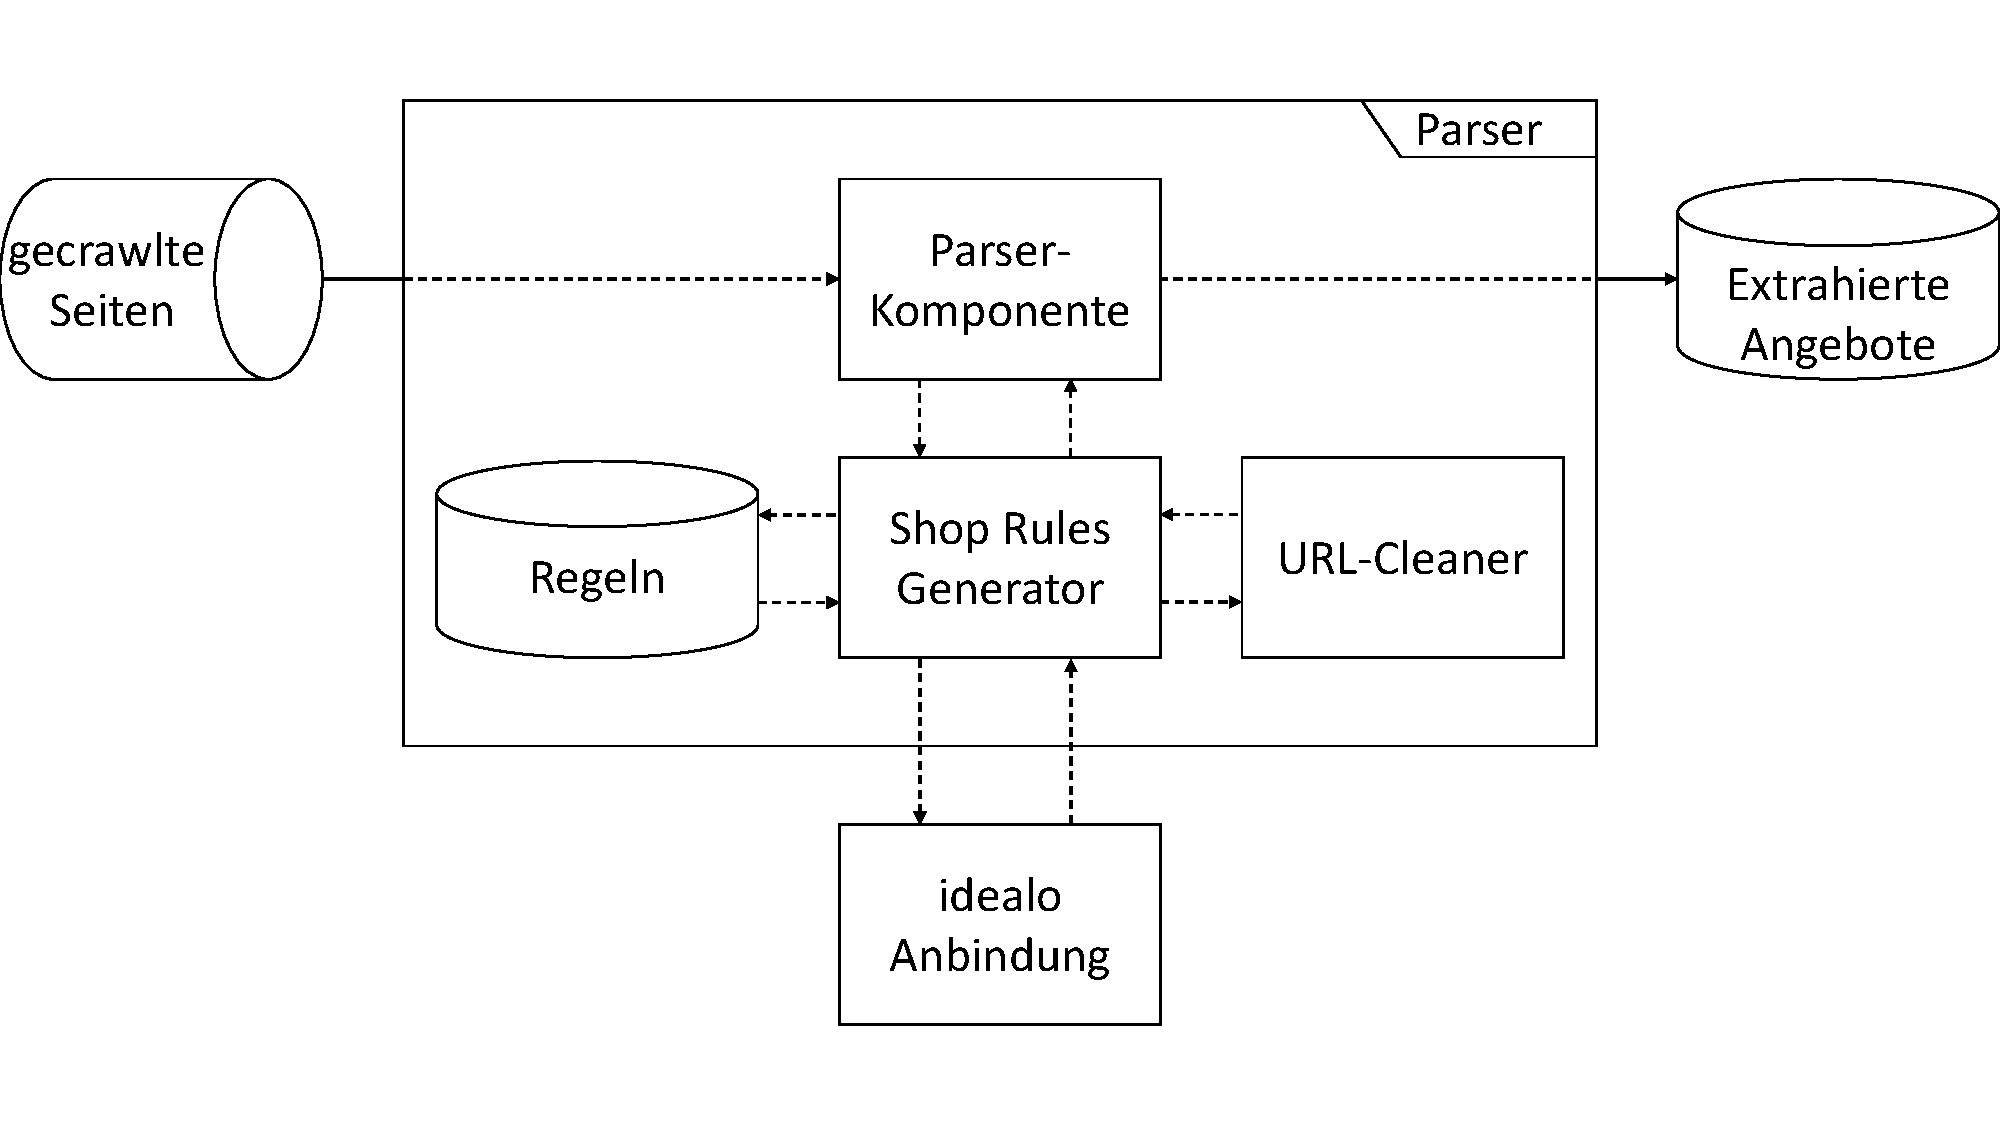
\includegraphics[width=\textwidth, trim=0 1.7cm 0 1.7cm, clip]{resources/Architektur-Parser.pdf}
    \caption{Architektur des Parsers}
    \label{fig:architektur-parser}
\end{figure}

\subsection{Die Funktionsweise der Parser-Komponente}
\label{subsec:funktionsweise-parser}

Die Parser-Komponente erhält ihre Eingaben, indem sie Nachrichten aus einer Queue konsumiert.
Eine Nachricht enthält eine vom Crawler heruntergeladene Webseite.
Der Crawler sendet zusätzlich zu jeder Seite die Webadresse und die Identifikationsnummer des zugehörigen Shops.
Nach dem Erhalt einer Nachricht, lädt der Parser vom SRG die Extraktionsregeln für den entsprechenden Shop.
Sollten die Regeln noch nicht existieren, wartet der Parser solange, bis die Regeln vom SRG erstellt wurden.
Sobald der Parser die Regeln empfangen hat, werden die Produktattribute aus der gecrawlten Seite extrahiert.
Die extrahierten Daten werden abschließend in einer Datenbank normalisiert gespeichert.

Der Matcher greift später auf diese Datenbank für den Vergleich zu.

\subsection{Die Funktionsweise des SRG}
\label{subsec:funktionsweise-srg}

Der Shop Rules Generator gibt auf Anfrage die Regeln für einen beliebigen Shop zurück.
Sollten die Regeln noch nicht existieren, werden sie generiert.

Während des Generierungsprozesses durchläuft der SRG mehrere Schritte.
Zuerst wird eine bestimmte Anzahl von Angeboten aus der idealo-Datenbank geladen.
Dies erfolgt über einen von idealo zur Verfügung gestellten API-Endpoint, welcher den Datenbankzugriff über eine
REST-Schnittstelle kapselt.
Dies hat den Vorteil, dass wir die Infrastruktur von idealo nutzen können und keine Kopie der Angebotsdaten
lokal speichern müssen.

Zu jedem dieser Angebote liegen die Webadresse für das Angebot, sowie die  Informationen über die in
Kapitel~\ref{subsec:technische-anforderungen-parser} genannten Produktattribute vor.
Außerdem wird für jedes Angebot das dazugehörige HTML-Dokument heruntergeladen.

Um die Server der Onlineshops nicht mit zu vielen Anfragen auf einmal zu strapazieren, wird zwischen jedem
Herunterladen einer Angebotsseite eine fest definierte Zeit gewartet.

Für die Menge der heruntergeladenen HTML-Dokumente ist bekannt, um welche Angebote es sich handelt und welche
konkreten Produktattribute erwartet werden.
Dieses Wissen wird für das Anlernen der Regeln genutzt.
Dazu werden die Werte aller Produkteigenschaften in dem HTML-Dokument gesucht.
Für jedes Vorkommnis eines Produktattributes wird eine Regel erstellt, die den Fundort referenziert.
Nachdem alle Regeln gesammelt wurden, wird eine finale Regelmenge bestimmt.
Diese Regelmenge wird in der Regeldatenbank gespeichert und bei zukünftigen Anfragen direkt zurückgegeben.

\subsection{Der URL-Cleaner}
\label{subsec:urlcleaner}

Manche Onlinehändler manipulieren vor der Übermittlung ihrer Angebote an idealo die Links zu deren Angeboten.
Sie fügen zu den regulären Webadressen Trackinginformationen hinzu.
Mit Hilfe dieser Trackinginformationen können sie nachvollziehen, welche Kunden durch idealo auf deren Seite gelandet
sind.
Dies ist für die Shopbesitzer sehr wichtig, da sie somit die CPC-Abrechnung von idealo kontrollieren können.
Die im Rahmen der Anlernphase getätigten Webseitenaufrufe könnten diese Statistiken jedoch verfälschen.
Für idealo ist es deshalb sehr wichtig, dass die Trackinginformationen vor dem Aufruf der Website entfernt werden.

Dazu haben wir die URL-Cleaner-Komponente entwickelt, welche Adressen mit Trackinginformationen als Eingabe erwartet und
bereinigt zurück gibt.

Wir haben zwei mögliche Verfahren entdeckt, wie die Trackinginformationen in Angebotslinks eingefügt werden können.
Dies ist sowohl über Redirects als auch URL-Parameter möglich.
Der URL-Cleaner wendet deshalb zwei Strategien sukzessive an, um die Trackinginformationen zu entfernen:

Die erste Strategie bereinigt die URL von Redirects.
Dabei gibt es zwei mögliche Verfahren der Redirect-Dienste:
Beim ersten Verfahren leitet der zwischengeschaltete Server den Besucher anhand der mitgesendeten URL-Parameter auf
die korrekte Seite weiter.
Die ursprüngliche URL ist hierbei somit bereits in der Redirect-URL enthalten.
Das zweite Verfahren ist etwas schwieriger, da anstatt der Ziel-Adresse lediglich ein kryptischer String mitgesendet
wird.
Die Weiterleitung ist erst nach der serverseitigen Zuordnung des kryptischen Strings zur tatsächlichen Adresse möglich.

In der Tabelle~\ref{tab:redirect} sind zwei Beispiele abgebildet, wie solche Redirect-Links aussehen könnten.
Eine Mischform der beiden Varianten ist ebenfalls möglich.

\begin{table}[h]
    \centering
    \begin{tabular}{ l | l }
        Redirect mit URL-Parameter                  &   cptrack.com/?redir=www.shop.de/product1\\
        Redirect mit krypt.\ Identifikationsstring   &   bit.ly/2Kqyrz2
    \end{tabular}
    \caption{Beispiele der Redirect-Verfahren}
    \label{tab:redirect}
\end{table}

Für das erste Redirect-Szenario wird die übergebene URL zunächst encodiert.
Anschließend wird die Root-Url des Shops in der encodierten URL gesucht und alles davor entfernt.
Für das zweite Szenario haben wir keine zufriedenstellende Lösung finden können.
Allerdings erkennt der URL-Cleaner jedoch, dass er mit diesem Fall nicht umgehen kann, da die Root-URL des Shops
nicht in der encodierten URL enthalten ist.

\begin{table}[h]
    \centering
    \begin{tabular}{ c }
        http://www.shop.de/product?\textbf{partner=idealo}?pid=96
    \end{tabular}
    \caption{URL mit parameterbasierten Trackinginformationen}
    \label{tab:trackparameter}
\end{table}

Die Tabelle~\ref{tab:trackparameter} zeigt eine Beispiel-URL mit parameterbasierten Trackerinformationen.
\textit{(Diese wurden fett hervorgehoben).}
Dabei können ebenfalls Parameter enthalten sein, welche nicht für das Tracking verwendet werden.

Um die parameterbasierten Trackerinformationen zu entfernen, werden alle Schlüssel-Wert-Parameterkombinationen
gelöscht, deren Schlüssel in einer vorher angelegten Liste vorkommen.
Diese Liste enthält alle Tracker-Schlüsselnamen, die bei einer manuellen Recherche über mehrere hundert Shops
häufiger vorgekommen sind.

Nachdem beide Strategien angewandt wurden, wird die bereinigte URL zurückgegeben.

\subsection{Das Erstellen von Selektoren}
\label{subsec:erstellen-von-selektoren}

Nachdem nun die allgemeine Vorgehensweise des Parsers und des Shop Rules Generators beschrieben wurden, geht es nun
konkret um das Erstellen von Selektoren.
Ein Selektor ist dabei wie eine Art Pfad und zeigt auf ein Element innerhalb der hierarchischen HTML-Struktur.
Wir kategorisieren die HTML-Elemente anhand dessen, wo das gesuchte Produktattribut steht.
Jedes HTML-Element wird durch ein Tag beschrieben.
Es gibt nun drei mögliche Orte, an denen das Produktattribut stehen kann: innerhalb eines Tags, in der Tag-Beschreibung
oder im Javascript.
Im nachfolgenden wird anhand eines Beispiels erklärt, wie die Regeln für jeden Typ erstellt werden.
Die EAN ist ein wichtiges Attribut, da es das Matching vereinfacht.
Wir wollen daher für unsere Beispiele jeweils einen Selektor für die EAN 9332721000108 erstellen.

\subsubsection{Das Erstellen von Text-Selektoren}
\label{subsubsec:erstellen-von-text-selektoren}

Wenn der gesuchte Wert in der Browser-Visualisierung der HTML-Seite enthalten ist, so lässt sich dafür ein
Text-Selektor bauen.
Dieser Selektor besteht zunächst lediglich aus einem eindeutigen CSS-Selektor, welcher minimal lang ist.
Eindeutig in diesem Kontext bedeutet, dass er nur auf das konkrete Element zeigt.
Diese Unterscheidung ist wichtig, da CSS-Selektoren auch so gebaut werden können, dass sie auf mehrere passende
Elemente zeigen.
Das Aufbauen des CSS-Selektors ist der "Copy selector"-Funktionalität der Entwicklerkonsole des Chrome-Browsers
nachempfunden.
Im Grundprinzip traversiert man ausgehend von dem Startelement über die Vater-Beziehung in der
DOM-Hierarchie Richtung Wurzel und speichert sich zu jedem Level die Information, das wievielte Kind das aktuelle
Element ist.
Für das obige Beispiel würde der Text-Selektor wie folgt aussehen: XXX TODO XXX BEISPIEL MIT ID NEHMEN!

\subsubsection{Das Erstellen von Description-Selektoren}
\label{subsubsec:erstellen-von-description-selektoren}

Während unserer Recherchen ist uns häufig eine leicht abgewandelte Form aufgefallen, bei der das gewünschte Attribut
in der Tag-Beschreibung anstatt im Inhalt des Tags stand.
Die Tag-Beschreibung ist nicht Bestandteil der Browser-Visualiserung.

Auch der Description-Selektor besteht wieder aus einem CSS-Selektor, welcher analog zu dem Text-Selektor aufgebaut ist.
Des Weiteren ist jedoch auch der Attributname Bestandteil des Selektors und hilft bei der Auswahl des korrekten
Schlüssel-Wert-Paares bei der Extraktion.

Mit Hilfe dieses Selektors lassen sich auch die Schema.org-Spezifikationen abbilden, insofern der Shop diese befolgt.
Um den Description-Selektor noch etwas flexibler zu machen und weniger starr an die Hierarchie des DOMs anzulehnen,
erstellen wir zusätzlich noch einen zweiten Description Selektor für jedes Vorkommnis.
Dieser zweite Selektor besitzt einen anderen CSS-Selektor, welcher sich nicht an der Hierarchie orientiert, sondern
an allen anderen Schlüssel-Wert-Paaren aus der Beschreibung des Tags.

Die beiden resultierenden Description-Selektoren sehen daher wie folgt aus:
XXX TODO XXX
XXX TODO XXX

\subsubsection{Das Erstellen von Script-Selektoren}
\label{subsubsec:erstellen-von-script-selektoren}

Die Text-Selektoren und die Description-Selektoren beziehen sich beide auf das DOM .
Der Script-Selektor unterscheidet sich dahingehend und bezieht sich auf die auf der Seite enthaltenen
Javascript-Einbindungen.
Viele Content-Management-Systeme verwenden Javascript für die Abspeicherung der Produktinformationen.
Auch JSON-LD, ein ähnlicher Standard wie Schema.org, verwendet spezielle Javascript-Tags für das Markieren von
Produktinformationen.
Dies macht es für uns sehr relevant, auch für diese Fälle ein Schema für den Selektoraufbau zu entwickeln.
Der Script-Selektor ist etwas komplizierter als die bereits vorgestellten Lösungen.

Bereits bei dem Text-Selektor als auch beim Description-Selektor haben wir festgestellt, dass die Hierarchie
innerhalb des HTML-Dokumentes sehr hilfreich ist.
Wir haben daher den Ansatz übernommen und erzeugen innerhalb des Javascript ebenfalls eine Hierarchie.
Der Script-Selektor besteht daher aus drei Teilen:
\begin{enumerate}
    \item dem CSS-Selektor, welcher innerhalb des DOMs zum entsprechenden Script-Element navigiert
    \item dem Block-Path, welcher innerhalb des Javascriptes zum korrespondierenden Block navigiert
    \item dem JsonPath, welcher ein XPath ähnlicher Pfad zu dem gewünschten Wert ist
\end{enumerate}

Der CSS-Selektor wird wieder analog zu dem Text-Selektor aufgebaut.

Der Beginn eines Blockes wird durch das Startsymbol \{ und das Ende durch das Endsymbol \} markiert, wobei eine
öffnende Klammer eine schließende Klammer verlangt und nur Blöcke betrachtet werden, bei denen die Anzahl der
öffnenden Klammern der der Schließenden entspricht.
Ein Block stellt zusammengefasst einen Codeschnipsel dar, der als JSON-Objekt interpretiert werden könnte.

Der Pfad wird letztendlich durch eine Tiefensuche durch die Blöcke des Javascript erstellt, was es ermöglicht auch
verschachtelte Konstrukte abzubilden.

Der JsonPath dient im letzten Schritt dazu, in dem interpretierten JSON-Objekt zu navigieren, um den gesuchten Wert
zurückzugeben.
JSON-Objekte bestehen aus weiteren Objekten, Arrays oder Attributen.
Für die Generierung des JSONPaths wird daher ebenfalls eine Tiefensuche innerhalb des Blocks angewandt.

Schlussendlich entsteht für das obige Beispiel folgender Script-Selektor:
XXX TODO XXX

\subsection{Eine generische Verbesserung aller Selektoren/ Die Trimming-Funktion}
\label{subsec:generische-verbesserung}

Für die Erstellung der obigen Selektoren sind wir bisher davon ausgegangen, dass der gesuchte Wert das einzige ist,
was in dem entsprechenden Feld enthalten ist.
Dies ist tatsächlich nur selten der Fall, so dass wir eine generische Verbesserung für alle Selektoren eingebaut haben.
Diese Verbesserung besteht in einer Art Trimming-Funktion, welche eine bestimmte Anzahl von Zeichen links und rechts
entfernt.
Somit werden auch Fälle wie in Abbildung X abgedeckt.
Der daraus resultierende Selektor sieht dadurch wie folgt aus:
XXX TODO XXX

\subsection{Die Bewertungsfunktion}
\label{subsec:bewertungsfunktion}

Mit der Vielfalt an Selektorenarten und der gesteigerten Flexibilität durch die Trimming-Funktion werden sehr viele
Selektoren erstellt.
Durch die gesteigerte Flexibilität fügt man jedoch auch ein "Rauschen" zu den Selektoren hinzu.
Das bedeutet, dass nun auch Selektoren erzeugt werden, welche nur selten vorkommen.
Sie werden für ein Angebot passend erzeugt, sind jedoch für die restlichen nicht korrekt und produzieren falsche
Ergebnisse.
Um diesen Umstand entgegenzuwirken, wurde eine Bewertungsfunktion eingeführt, welche nach dem Generieren aller
Selektoren ausgeführt wird.
Dazu wird erneut über alle von idealo geladenen Angebotsinformationen iteriert und für jeden Selektor bestimmt, wie
oft dieser ein richtiges Ergebnis extrahiert hat.
Richtig bedeutet in diesem Kontext, dass der extrahierte Wert genau dem Wert aus den Angebotsinformationen entspricht.
Dabei wird für jeden Match der Score erhöht und für jeden Mismatch der Score verringert.
Eine Ausnahme bildet jedoch der leere String "".
In diesem Fall belassen wir den Score so wie er ist.
Wir haben uns dazu entschieden, da wir bei dem leeren String erkennen können, dass die Regel nichts produziert hat.
Wenn die Regel jedoch etwas Falsches zurückliefert, können wir uns später nicht mehr sicher sein, ob dies schlichtweg
falsch, oder etwas Neues ist.
Abschließend wird dieser Score normalisiert, das heißt er wird auf eine Skala von 0 bis 1 abgebildet, indem durch die
Anzahl der Vorkommnisse der einzelnen Attribute in den Angeboten dividiert wird.
Der Score 1 ist hierbei besser und bedeutet, dass in allen Fällen der richtige Wert extrahiert wurde.

Nun verfügt jeder Score über eine genaue Metrik, wie gut der Selektor ist.
Um das Rauschen zu minimieren, werden nun alle Selektoren, deren normalisierter Score sich unter einem bestimmten
Schwellwert befindet verworfen.
Alle übrigen Selektoren werden in geordnet pro Produktattribut in der shop-spezifischen Regel gespeichert.

Die Parser-Komponente verwendet den Score ebenfalls für das Evaluieren des besten Extraktionskandidaten.
Dazu wird nach allen gefunden Werten gruppiert und die normalisierten Scores aufaddiert.
Der Wert mit dem höchsten resultierenden Score wird zurückgegeben.

\begin{comment}
    Implementierung: Um den nichtfunktionalen Anforderungen, insbesondere der Skalierbarkeit und Parallelität zu genügen, arbeitet die
    Parser-Komponente mit mehreren Threads und kann somit mehrere gecrawlte Seiten gleichzeitig verarbeiten.
    Zudem wurden Cache-Mechanismen verwendet, um die Anfragen an den SRG zu minimieren.
\end{comment}